
\index{Sch\"omann, Klaus}

\paragraph{Research Team}
Klaus Sch\"omann (Professor), Anette Fasang (Doctoral Fellow), Paula Aleksandrowicz (Doctoral Fellow).

Germany faces a dual demographic challenge in the next 15 years. This consists in a considerable aging of the working-age population and of the total population, along with a shrinking size of the population of working-age. The size of the working-age population is projected to decline from 50 to 40 million people in 2020. Increasing the participation in employment of older workers is an important consequence of this demographic trend. To enable similar potentials of economic growth in the coming years not only more ``silver workers'' will have to work from each birth cohort, but the extension of the working live becomes likely scenario which is subject of our research interest in the field of productive aging. 

 Our second research theme deals with the links and exchangeability between human capital and social capital. We analyze the potential to increase voluntary work or civic engagement of older workers as the average life expectancy and fitness in older age increase. Thereby we assess the reversibility of retirement transitions and new combinations of market and non-market work in Western societies. 

 The part of sociology in the subproject "Learning" within the framework of the joint BMBF project concerns the area of learning participation and opinions of learning and their match with learning strategies and the learning culture of within a firm under the demographic aging of the employees and management. 

\begin{figure}[h]
  \begin{center}
    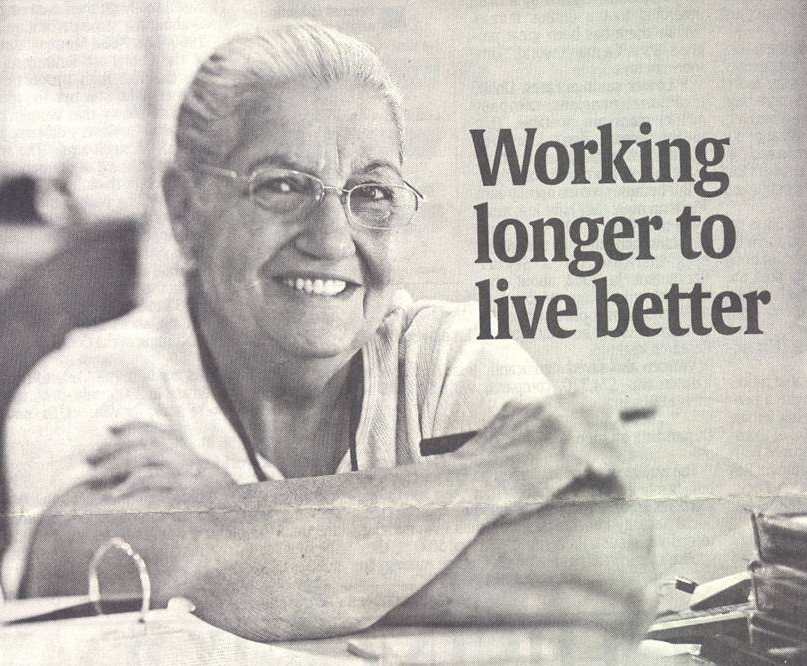
\includegraphics[width=7.5cm]{profKlausSchoemann-fig2.jpg}
    \caption{A challenging research agenda for life course sociology (Source: USA today 14.9.2006).}\label{fig2:profKlausSchoemann}
   \end{center}
\end{figure}

\textbf{Research Highlights 2006}

 Based on our first telephone survey of employees in part-time retirement in one firm we have produced a report on the results for the company executives. We have already achieved a faster turnaround from collecting survey data ourselves to data analysis and publication of results. The finding that even the retirement transition might be a transition, that can be reversed was received with some enthusiasm in the company as they are looking already for means to rehire some of their previous employees sent into early retirement. Similarly the combination of civic engagement of the enterprise and its former employees might constitute an interesting future potential of cooperation beyond the traditional employment relationship of dependent full-time employees in this firm. 

 Additionally we started to cooperate with the ``European initiative for the rights of future generations'' in the field of social policies. 


\paragraph{Collaborations}
\begin{itemize}
\item OECD Department of Employment and Social Affairs
\item Universit\'e Paris I, MATISSE \\ Maitre de Conf\'erences \\ Christine Erhel
\item University of V\"axj\"o  \\ Prof. Dominique Anx\"o 
\item OSA Institute for Labour Studies  \\ Dr. Frank Tros 
\item University of North Carolina at Chapel Hill  \\ Prof. Dr. Arne Kalleberg
\end{itemize}

\begin{bibunit}[apalike]
\nocite{*}
\putbib[profKlausSchoemann2]
\end{bibunit}


\paragraph{Grants}
\begin{itemize}
\item BMBF (PI: JCLL). K. Sch\"omann, C. Ro\ss nagel: subproject ``Learning / Training'' within the joint research project ``Effects of Matches/Mismatches between Aspects of Human and Social Capital, Corporate Strategy and Work Organization on the Physical and Mental Well-Being of Employees''. 
\item Consulting Project (PI: K. Sch\"omann, U. Staudinger): Retirement Processes in a Large Firm.
\item Consulting Project (PI: K. Sch\"omann): Evaluation of company-wide occupational health and safety trainings.
\item Executive Teaching for AutoUni in Wolfsburg by K. Sch\"omann.
\item DFG Travel Grant for Anette Fasang to present her first research results to the Sociology department at Yale, USA.
\item Grant by the European Sociological Association for Sara Geerdes for participation in a Summer School on Migration in Milano, Italy.
\end{itemize}